\documentclass{beamer}
\mode <presentation>
{
    \usetheme{boxes}
    \usecolortheme{crane}
    \setbeamercovered{transparent}
}
\definecolor{craneorange}{RGB}{220,197, 90}

\usepackage[absolute,overlay]{textpos}
\usepackage{pgf,pgfarrows,pgfnodes}
\usepackage[english]{babel}
\usepackage{lmodern}
\usepackage{newcent}
\usepackage{amsmath}
% math extension - one probably wants to use symbols like '[' (written as '$[$')
\usepackage{ucs}
%\usepackage[utf8]{inputenc}
%\usefonttheme{structuresmallcapsserif}

% utf8x does not work with xetex
\usepackage{ifxetex}
\ifxetex
\else
        \usepackage[utf8x]{inputenc}
\fi

\usepackage[normalem]{ulem}


\setlength{\TPHorizModule}{1mm}
\setlength{\TPVertModule}{1mm}
\newcommand{\WorkInProgress}{%
\begin{textblock}{14}(120.0,75.7)

\includegraphics[height=0.7cm]{./pics/workinprogress.jpg}
\end{textblock}
  }

%\setbeamercolor{background canvas}{bg=
\includegraphics[width=\textwidth]{./pics/wolf.png}}

\title{IT asset management with GLPI}
\author{\href{http://www.glpi-project.org/}{GLPI project}}
\subject{GLPI - the IT asset management solution}
\keywords{IT asset management, Inventory, GLPI}

\date{July 2011}
%\titlegraphic{GLPI}
%subtitle{
\includegraphics[width=1.2cm]{./pics/fusioninventory-logo.png}}
\institute{
\includegraphics[height=4.2cm]{./pics/rmll2011.jpg}}
\author{ Gonéri Le Bouder and David Durieux }
\logo{
\includegraphics[height=0.7cm]{./pics/logos/glpi+fusinv_small.jpg}}

\AtBeginSection[] % Do nothing for \section*
{
    \begin{frame}<beamer>
        \frametitle{Outline}
    \tableofcontents[currentsection]
        \end{frame}
}


%%%%%%%%%%%%%%%%%%%%%%%%%%%%%%%%%%%%%%%%%%%%%%%
%%%%%%%%%%%%%%%%%%%%%%%%%%%%%%%%%%%%%%%%%%%%%%%
\begin{document}

\frame[plain]{\titlepage}

\begin{frame}
    \frametitle{About us: David Durieux}

    \begin{block}{IT management consultant}
        \begin{itemize}
        \item GLPI core-developer
        \item FusionInventory project co-leader
        \item Work at siprossii, Lyon area, France
        \end{itemize}
    \end{block}

\end{frame}



\begin{frame}
    \frametitle{About us: Gonéri Le Bouder}


    \begin{block}{Free software enthusiast}
        \begin{itemize}
        \item Debian Developer
        \item Perl Monger
        \item Former OCS Inventory developer
        \item FusionInventory project co-leader
        \item Work at TECLIB', Paris, France
        \end{itemize}
    \end{block}

\end{frame}


\section{What is GLPI for?}


\begin{frame}
    \frametitle{What is GLPI for?}

 \begin{columns}
 \begin{column}{0.35\textwidth}
         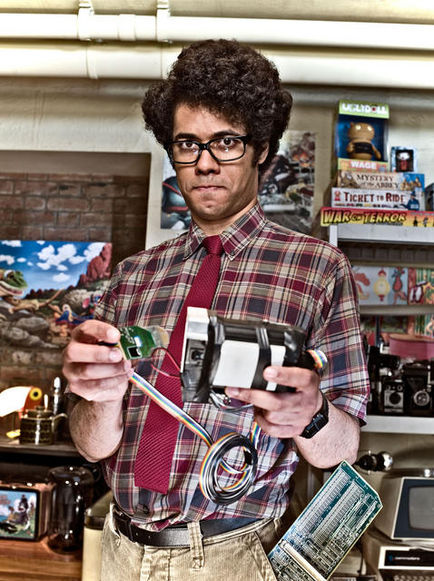
\includegraphics[height=7.5cm]{./pics/itcrowd.jpg}
 \end{column}
 \begin{column}{0.65\textwidth}
    \begin{block}{The IT crowd}
        \begin{itemize}
            \item How many server still run with 2GB of memory?
            \item Do we still have those old Toshiba laptops?
            \item Do our servers have the lastest security fixes?
        \end{itemize}
    \end{block}
 \end{column}
\end{columns}

 \end{frame}

\begin{frame}
    \frametitle{What is GLPI for?}

 \begin{columns}
 \begin{column}{0.1\textwidth}
         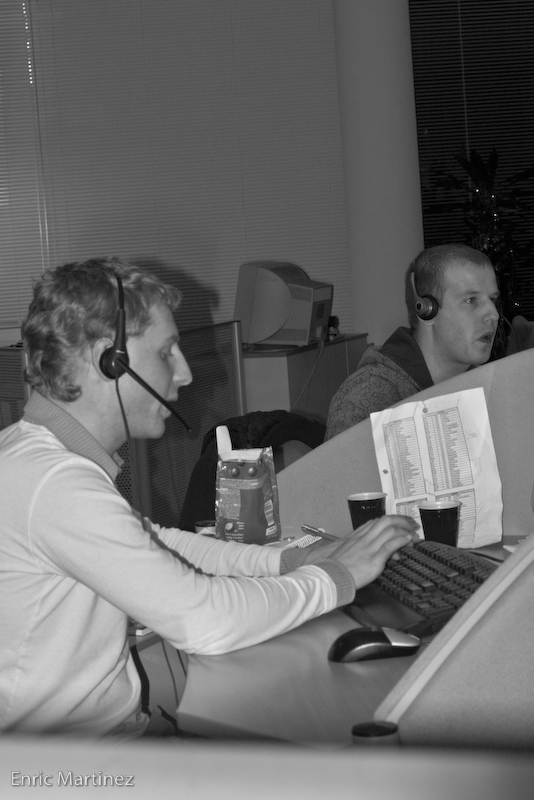
\includegraphics[height=7.5cm]{./pics/helpdesk.jpg}
 \end{column}
 \begin{column}{1\textwidth}

    \begin{block}{The Service Desk team}
        \begin{itemize}
            \item Is Mr Smith computer's harddrive full?
            \item What is my intervention planning?
            \item The printer ink cartridge is running \\
                low on the second floor!
        \end{itemize}
    \end{block}
 \end{column}
\end{columns}


\end{frame}

\begin{frame}
    \frametitle{What is GLPI for?}

 \begin{columns}
 \begin{column}{0.35\textwidth}
         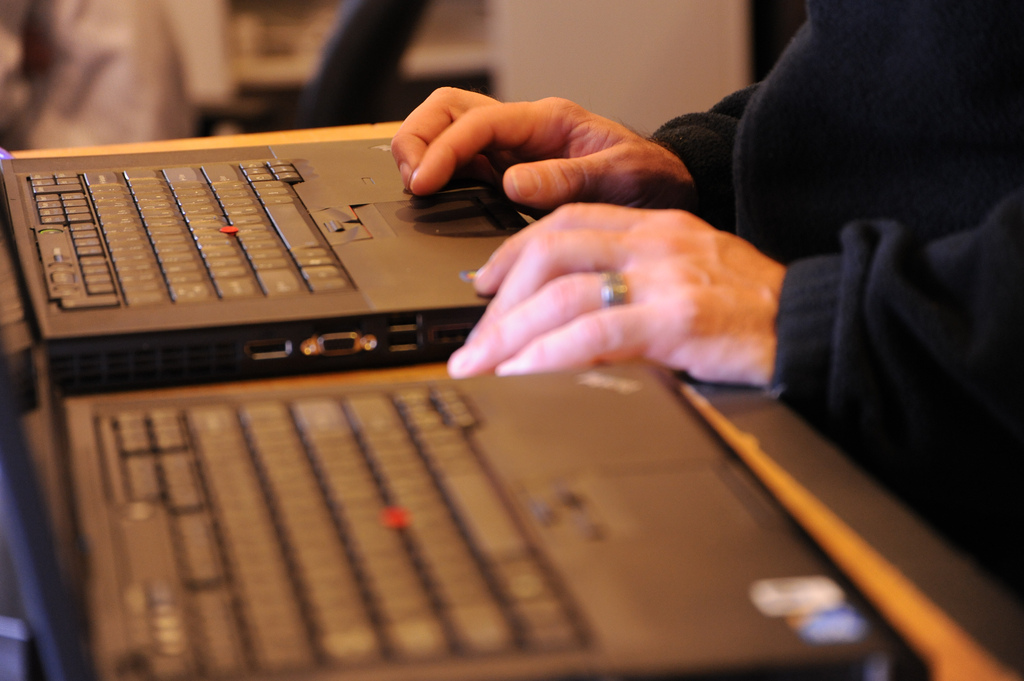
\includegraphics[height=7.5cm]{./pics/lenovo.jpg}
 \end{column}
 \begin{column}{0.65\textwidth}

    \begin{block}{The users}
        \begin{itemize}
            \item Why can't I print?
            \item Why can't I send email anymore?
            \item Are the IT guys really processing my request?
        \end{itemize}
    \end{block}
 \end{column}
\end{columns}

\end{frame}

\begin{frame}
    \frametitle{What is GLPI for?}

 \begin{columns}
 \begin{column}{0.15\textwidth}
         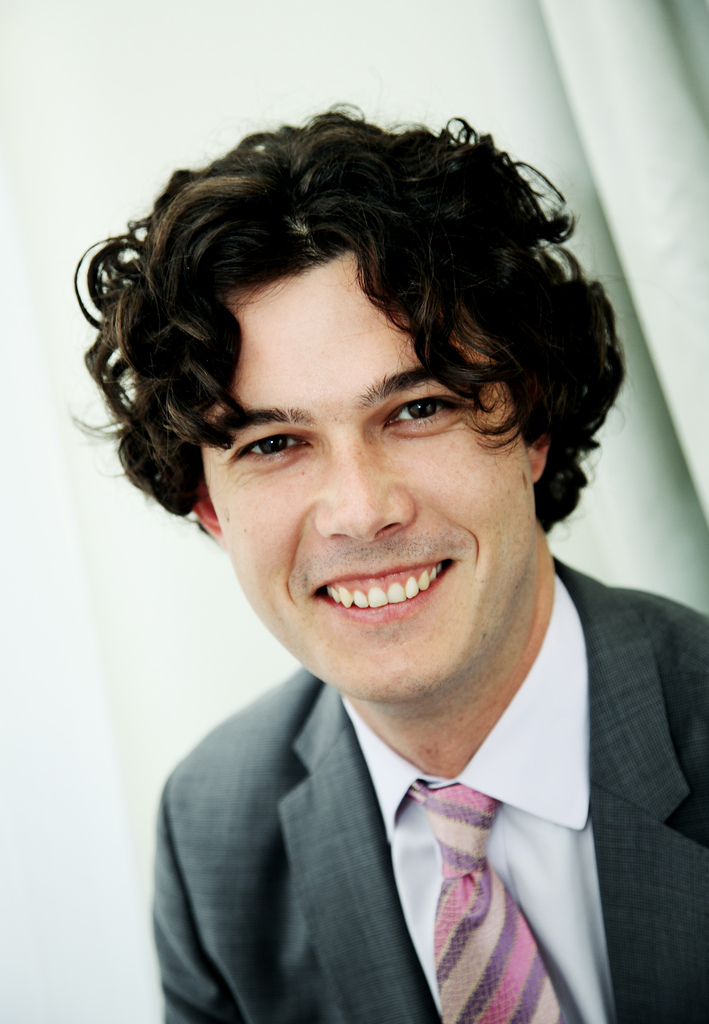
\includegraphics[height=8.5cm]{./pics/manager.jpg}
 \end{column}
 \begin{column}{1.25\textwidth}
    \begin{block}{The management}
        \begin{itemize}
            \item How many request per day processed by our support team?
            \item What is our users satisfaction's level?
            \item I need more dashboards!
        \end{itemize}
    \end{block}
 \end{column}
\end{columns}


\end{frame}


\begin{frame}
    \frametitle{What is GLPI for?}

 \begin{columns}
 \begin{column}{0.35\textwidth}
         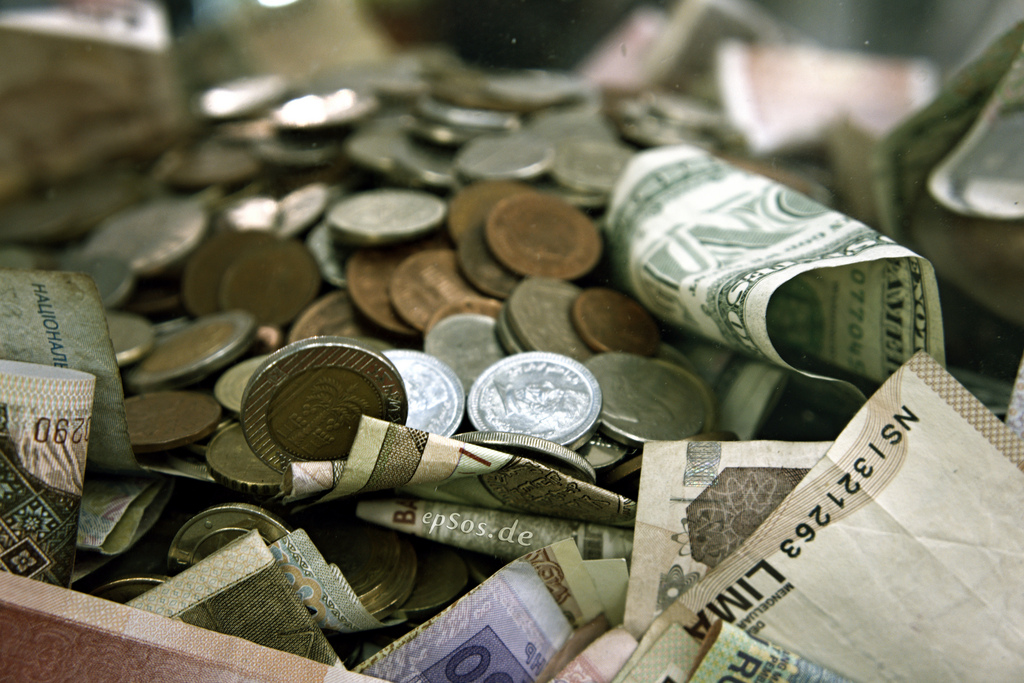
\includegraphics[height=7.5cm]{./pics/purchasing.jpg}
 \end{column}
 \begin{column}{0.65\textwidth}
    \begin{block}{The purchasing department}
        \begin{itemize}
            \item How much did we spend last year with IBM?
            \item Is the paternship with Oracle still running?
            \item How many and where are the assets bought with last year budget?
        \end{itemize}
    \end{block}
 \end{column}
\end{columns}
\end{frame}


\section{Installation / Architecture?}


\begin{frame}
    \frametitle{Installation}

%         \pgfputat{\pgfxy(-1,-3)}{\pgfbox[left,top]{
\includegraphics[height=2.5cm]{./pics/php-mysql.jpg}}}
    \begin{block}{Easy step}
        \begin{itemize}
            \item Common web application
            \item Very few OS dependencies
            \item Extract, run the wizard, done!
        \end{itemize}
    \end{block}


\end{frame}


\begin{frame}
    \frametitle{Architecture}

 \begin{columns}
 \begin{column}{0.34\textwidth}
    
\includegraphics[height=5.5cm]{pics/scale.png}
 \end{column}
 \begin{column}{0.90\textwidth}
    \begin{block}{How does it scale?}
        \begin{itemize}
            \item Existing large installation of GLPI \\
            {\small up to 130K computers inventoried}
            \item 1 million computers referenced so far and still growing
        \end{itemize}
    \end{block}
 \end{column}
\end{columns}
\end{frame}


\section{Collect your informations}

\begin{frame}

    \frametitle{Collect your information}

 \begin{columns}
 \begin{column}{0.34\textwidth}
    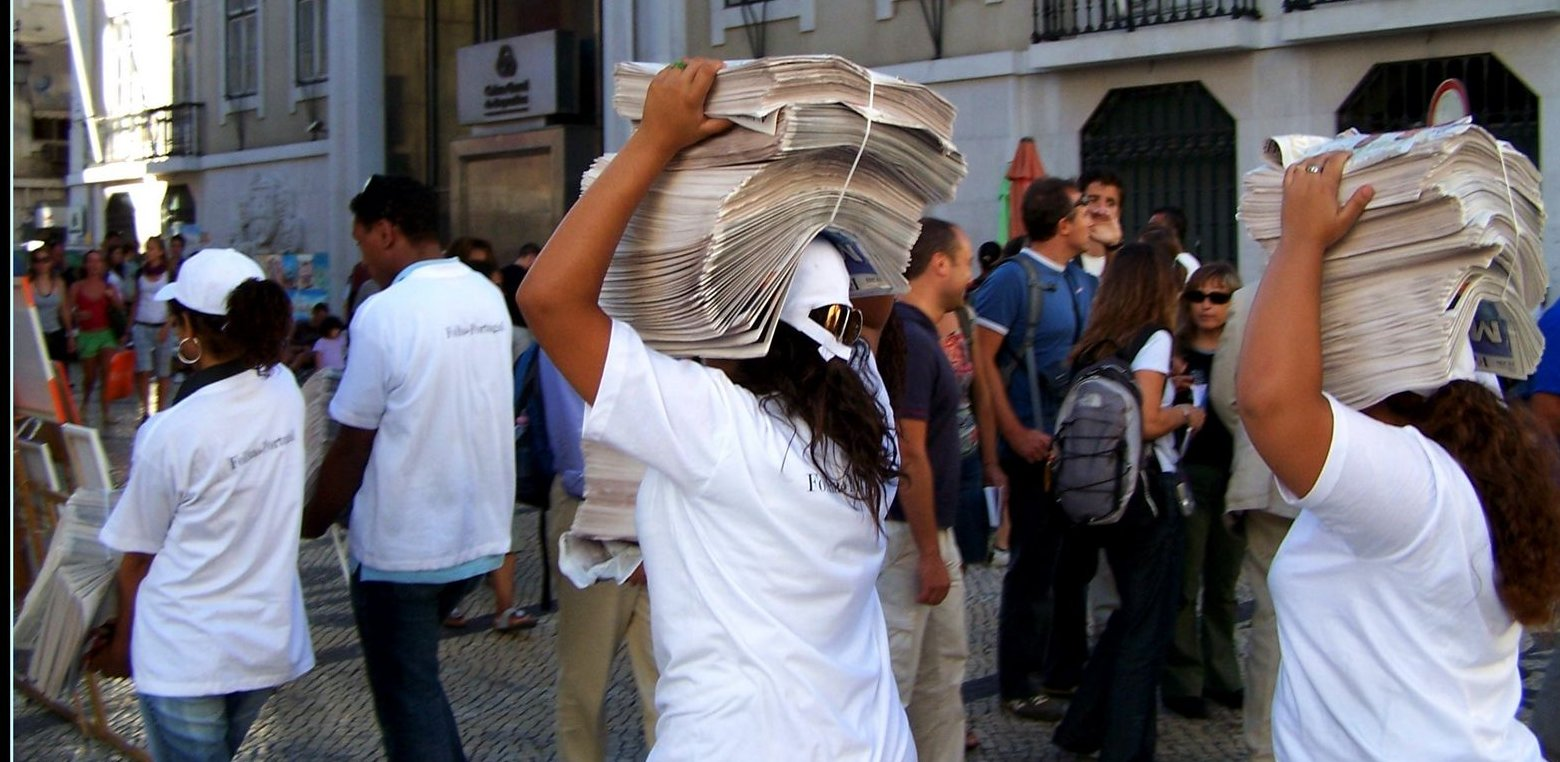
\includegraphics[height=6.5cm]{pics/information.jpg}
 \end{column}
 \begin{column}{0.90\textwidth}
 \end{column}
\end{columns}


\end{frame}



\begin{frame}

    \frametitle{Collect your information}

 \begin{columns}
 \begin{column}{0.34\textwidth}
    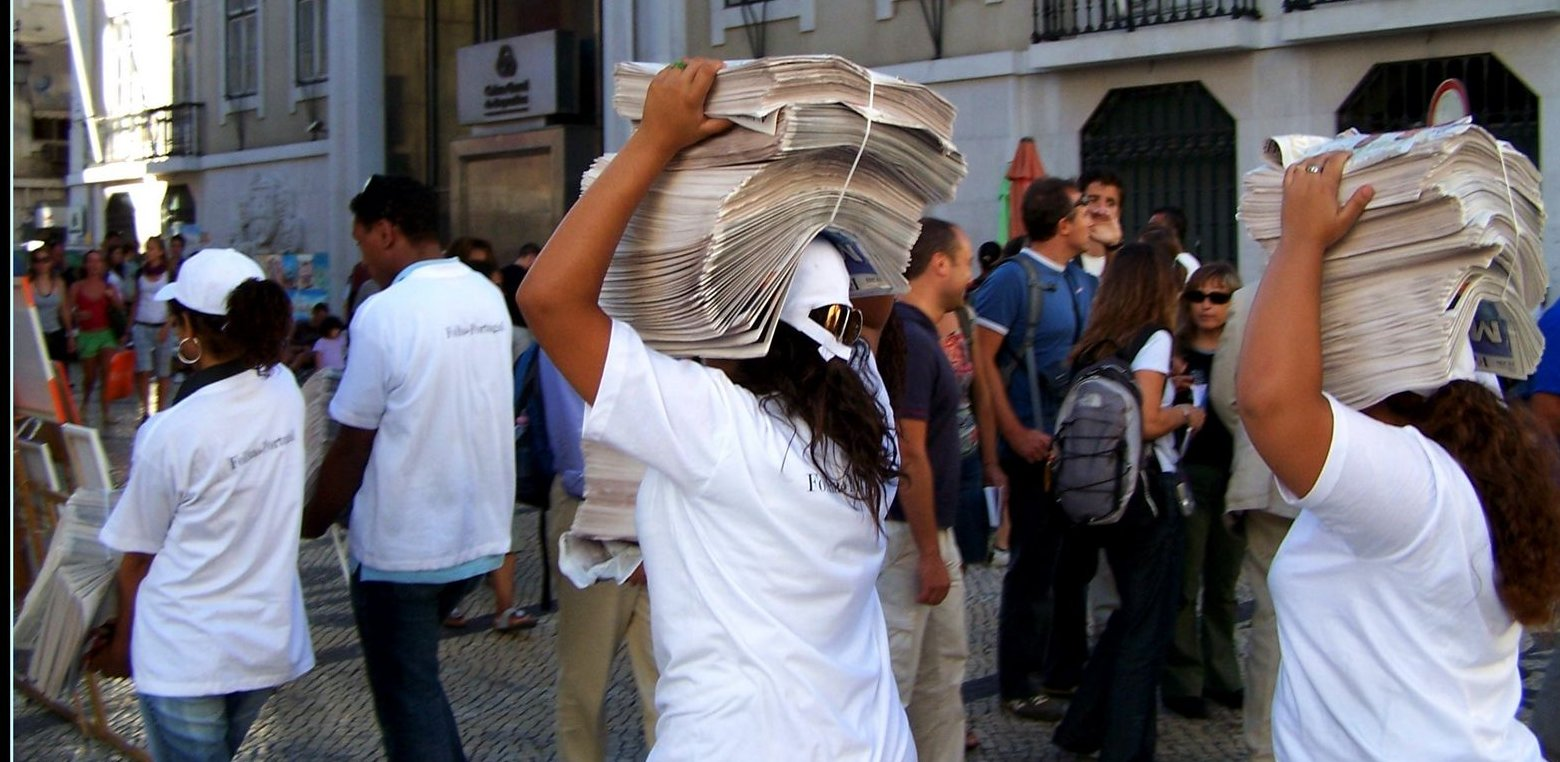
\includegraphics[height=6.5cm]{pics/information.jpg}
 \end{column}
 \begin{column}{0.90\textwidth}
    \begin{block}{Inputs}
        \begin{itemize}
            \item Desktop computers and server
            \item Network devices
            \item Data coming from legacy systems
            \item Financial informations
            \item ...
        \end{itemize}
    \end{block}

 \end{column}
\end{columns}


\end{frame}


\begin{frame}

    \frametitle{Network devices}


 \begin{columns}
 \begin{column}{0.15\textwidth}
         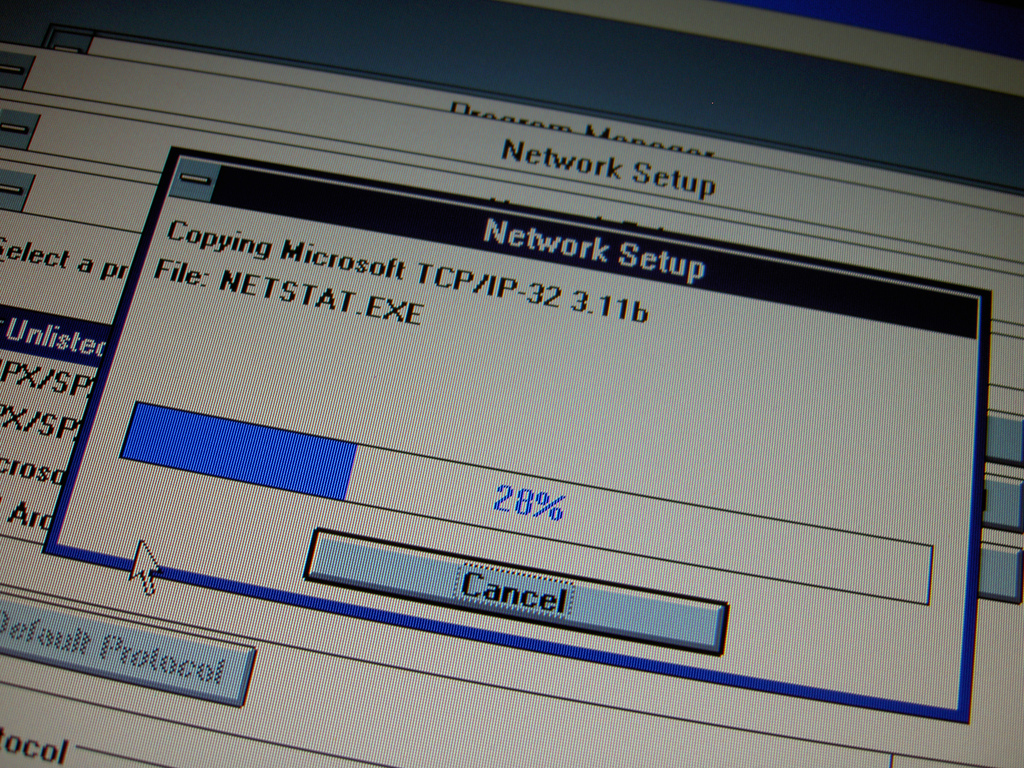
\includegraphics[height=8.5cm]{./pics/networking.jpg}
 \end{column}
 \begin{column}{1.25\textwidth}


    \begin{block}{Routers, switchs, printers... \\
    FusionInventory do it remotely for you}
        \begin{itemize}
            \item Nothing to install
            \item Network scan to identify asset
            \item Use SNMP to collect information
            \item ESX/ESXi/vCenter remote inventory
        \end{itemize}
    \end{block}

 \end{column}
\end{columns}
\end{frame}


\begin{frame}

    \frametitle{Network devices}


 \begin{columns}
 \begin{column}{0.15\textwidth}
         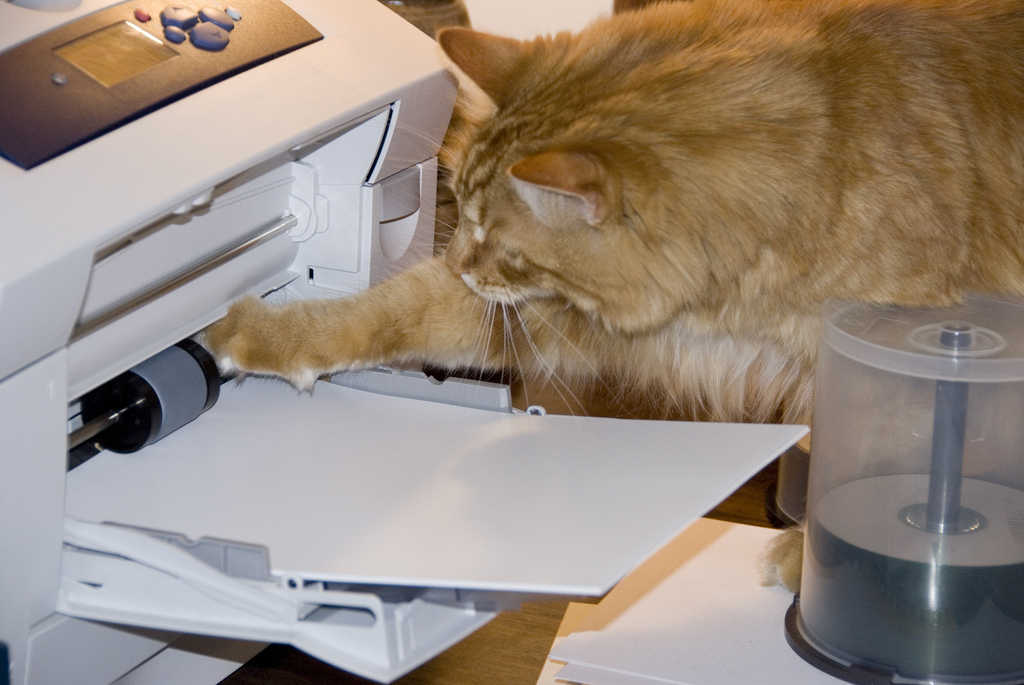
\includegraphics[height=8.5cm]{./pics/printer.jpg}
 \end{column}
 \begin{column}{1.25\textwidth}


    \begin{block}{printers}
        \begin{itemize}
            \item Cartridge ink levels
            \item Counters and statistics
        \end{itemize}
    \end{block}

 \end{column}
\end{columns}
\end{frame}


\begin{frame}


    \frametitle{GLPI, all in one}
 \begin{columns}
 \begin{column}{0.45\textwidth}
         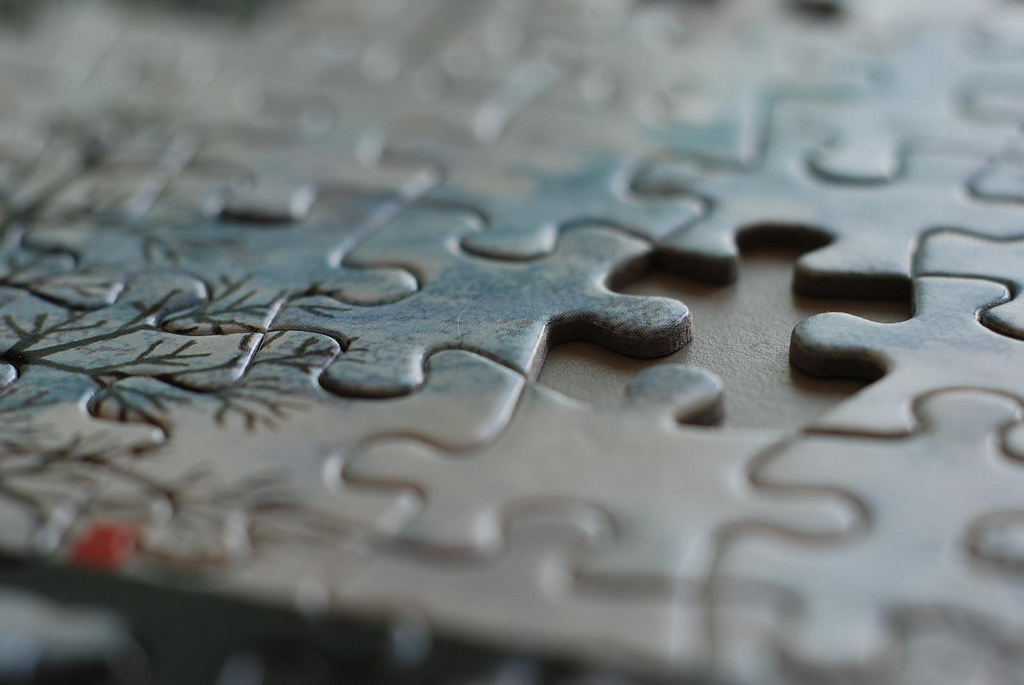
\includegraphics[height=7.5cm]{./pics/glpithelink.jpg}
 \end{column}
 \begin{column}{0.65\textwidth}
    \begin{block}{The asset timeline}
        \begin{itemize}
            \item Past: history
            \item Current: inventory
            \item Future: warranty, contracts
        \end{itemize}

    \end{block}

 \end{column}
\end{columns}
\end{frame}


\begin{frame}


    \frametitle{GLPI, all in one}
 \begin{columns}
 \begin{column}{0.45\textwidth}
         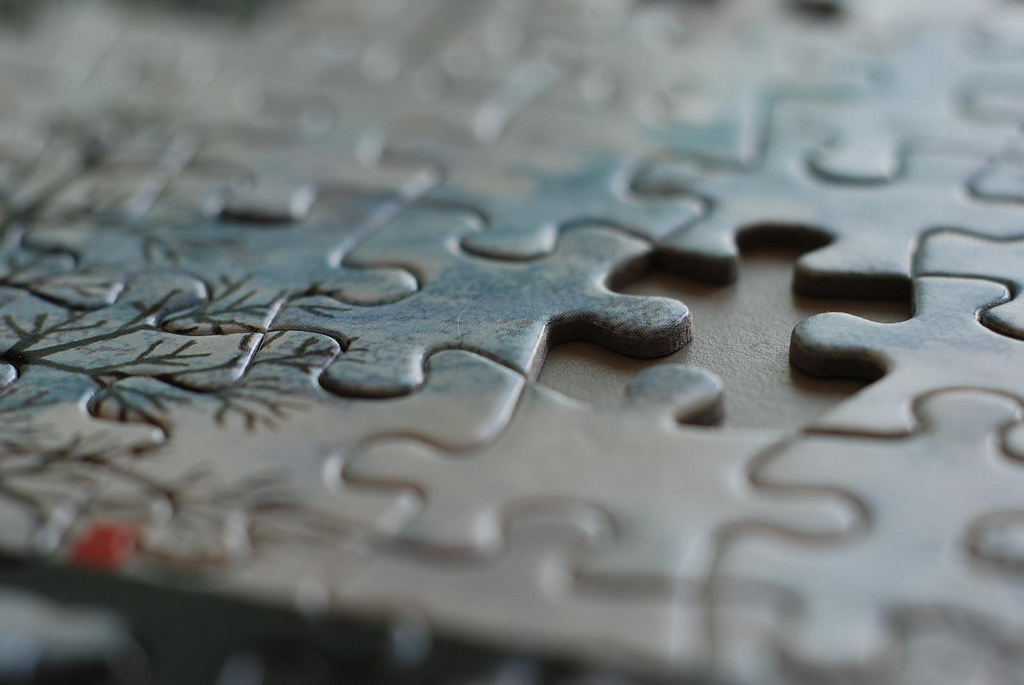
\includegraphics[height=7.5cm]{./pics/glpithelink.jpg}
 \end{column}
 \begin{column}{0.65\textwidth}
    \begin{block}{Helpdesk for everyone}
        \begin{itemize}
            \item Tickets on assets
        \end{itemize}

    \end{block}

 \end{column}
\end{columns}
\end{frame}

\begin{frame}


    \frametitle{GLPI, all in one}
 \begin{columns}
 \begin{column}{0.45\textwidth}
         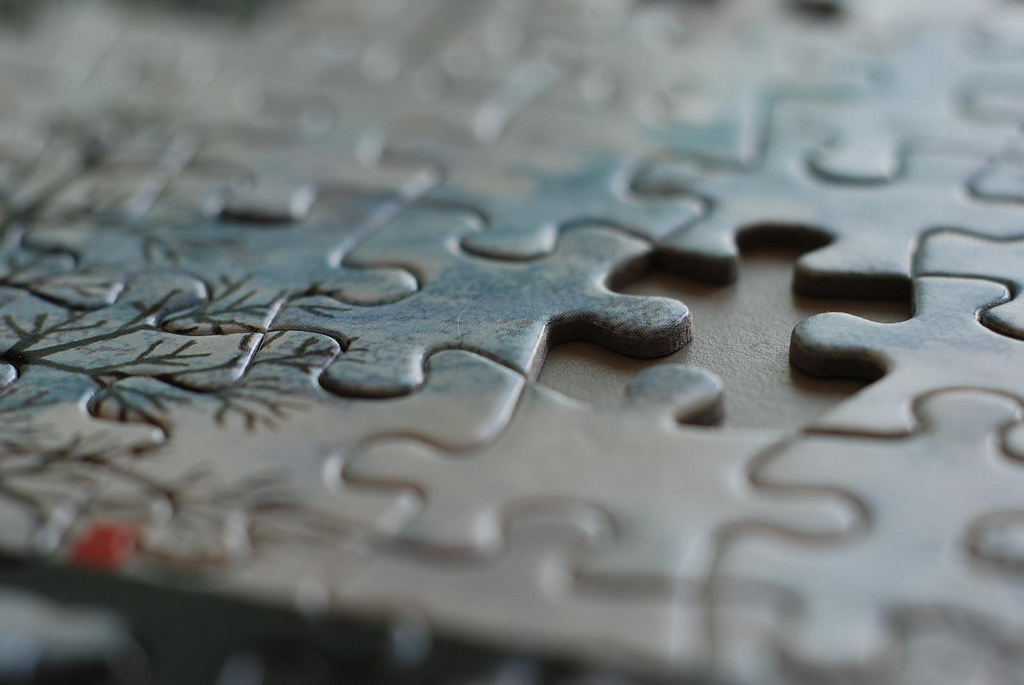
\includegraphics[height=7.5cm]{./pics/glpithelink.jpg}
 \end{column}
 \begin{column}{0.65\textwidth}
    \begin{block}{Accurate statistics}
        \begin{itemize}
            \item 25\% of last year laptops have harddrive failure !
            \item How many incidents are resolved by using VNC  ?
        \end{itemize}

    \end{block}

 \end{column}
\end{columns}
\end{frame}

\section{Authorisation}

\begin{frame}
    \frametitle{Authorisation}


 \begin{columns}
 \begin{column}{0.34\textwidth}
    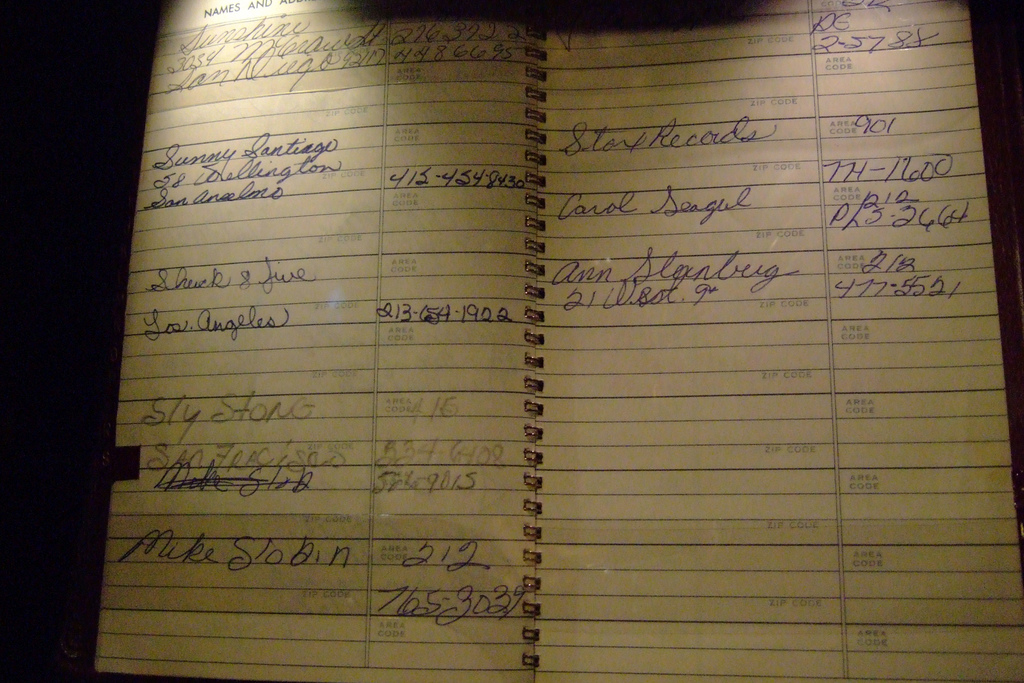
\includegraphics[height=6.5cm]{pics/addressbook.jpg}
 \end{column}
 \begin{column}{0.90\textwidth}
    \begin{block}{Native LDAP support}
        \begin{itemize}
            \item Strong LDAP integration
            \item LDAP v3 compatible \\
            {\small Active Directory, OpenLDAP ...}
        \end{itemize}
    \end{block}

    \begin{block}{Other authentication methods}
        \begin{itemize}
            \item POP3
            \item IMAP
        \end{itemize}
    \end{block}
 \end{column}
\end{columns}
\end{frame}

\begin{frame}
    \frametitle{Authorisation}


 \begin{columns}
 \begin{column}{0.34\textwidth}
    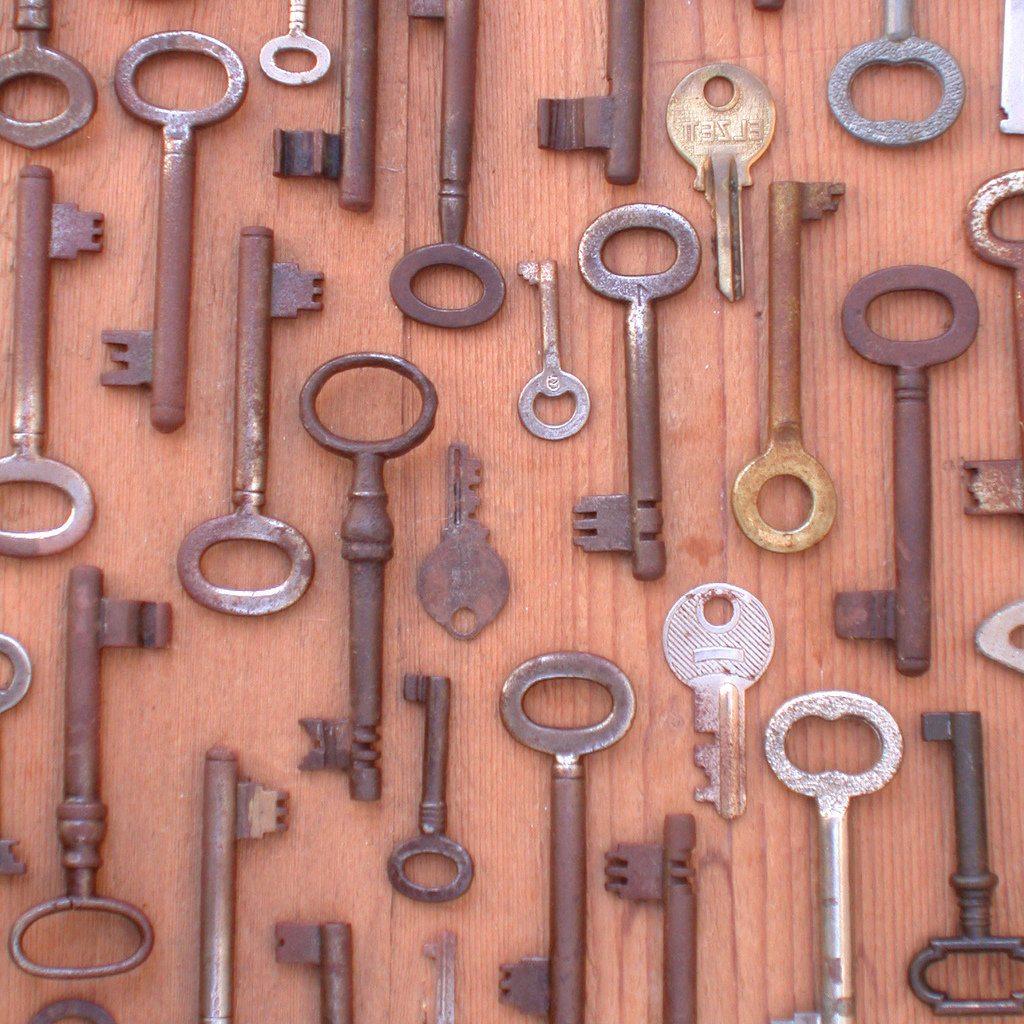
\includegraphics[height=10.5cm]{pics/sso.jpg}
 \end{column}
 \begin{column}{0.90\textwidth}
    \begin{block}{Single Sign On too!}
        \begin{itemize}
            \item WebSSO
            \item CAS
        \end{itemize}
    \end{block}
 \end{column}
\end{columns}

\end{frame}




\begin{frame}
\frametitle{Authorisation}
    \begin{block}{Entities}
        \begin{itemize}
            \item Independent administrative entity
            \item Can be mapped on your LDAP organisation
            \item Contain assets and tickets
        \end{itemize}

    \end{block}
\end{frame}


\begin{frame}
\frametitle{Authorisation}
    \begin{block}{Profile}
        \begin{itemize}
            \item More than 100 rights
            \item Habilitation : a profile on an entity
        \end{itemize}
    \end{block}
\end{frame}


\section{Service Desk}

\begin{frame}
\frametitle{Service Desk: the big picture}
\begin{columns}
\begin{column}{0.45\textwidth}
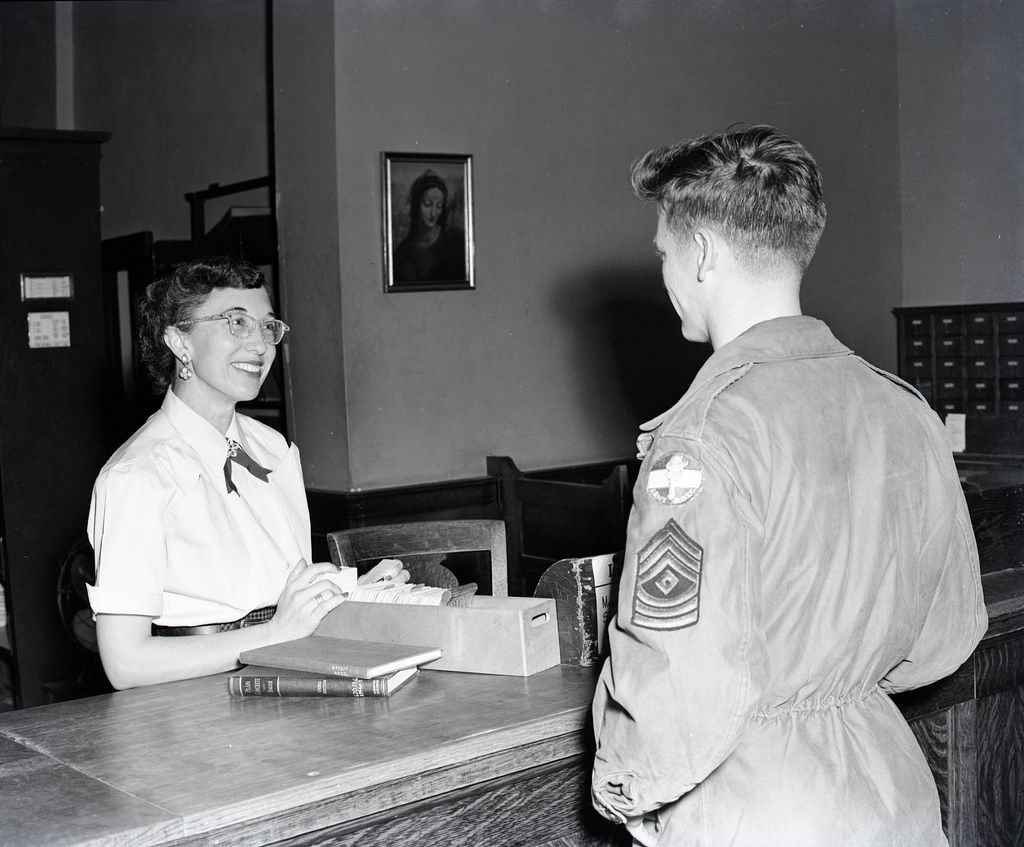
\includegraphics[height=7.5cm]{./pics/servicedesk.jpg}
\end{column}
\begin{column}{0.45\textwidth}
\end{column}
\end{columns}
\end{frame}



\begin{frame}


    \frametitle{Service Desk: the big picture}
 \begin{columns}
 \begin{column}{0.45\textwidth}
         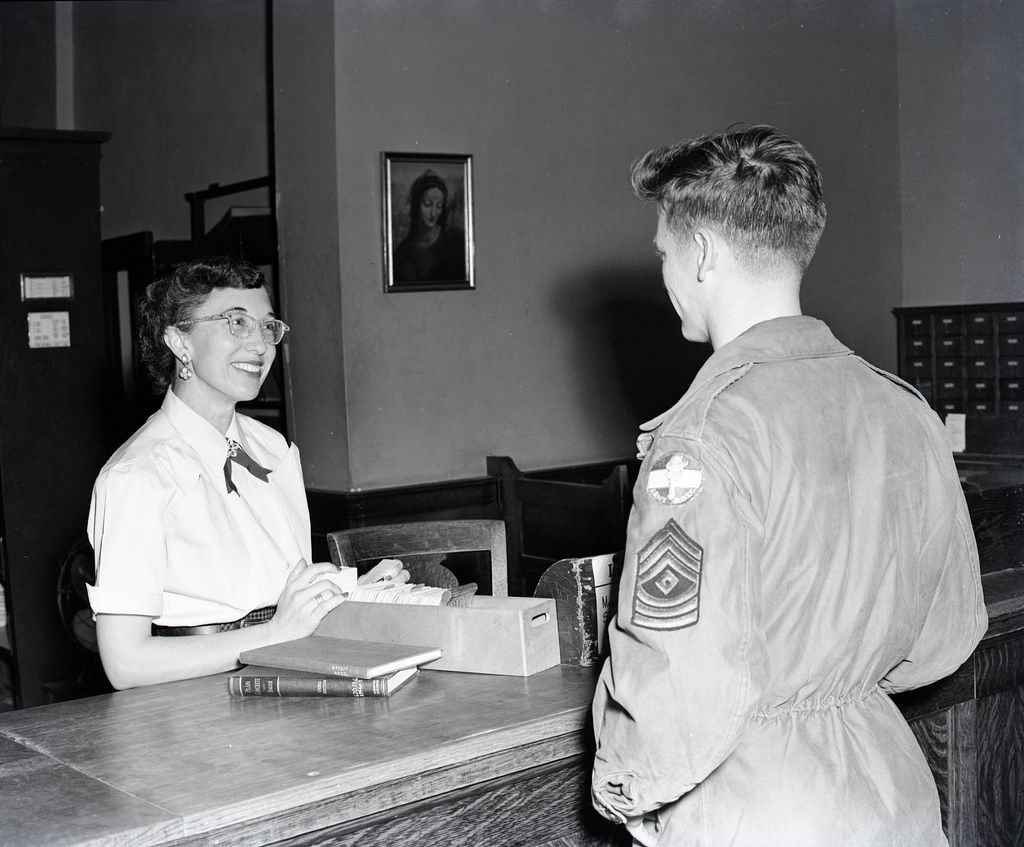
\includegraphics[height=7.5cm]{./pics/servicedesk.jpg}
 \end{column}
 \begin{column}{0.45\textwidth}
    \begin{block}{ITIL v1 compliant}
        \begin{itemize}
            \item SLA
            \item user satisfaction
            \item Incident management
            \item Business rules
            \item Notifications, multilingual support
        \end{itemize}

    \end{block}

 \end{column}
\end{columns}
\end{frame}

\begin{frame}

    \frametitle{Service Desk: the interfaces 1/2}

 \begin{columns}
 \begin{column}{0.45\textwidth}
         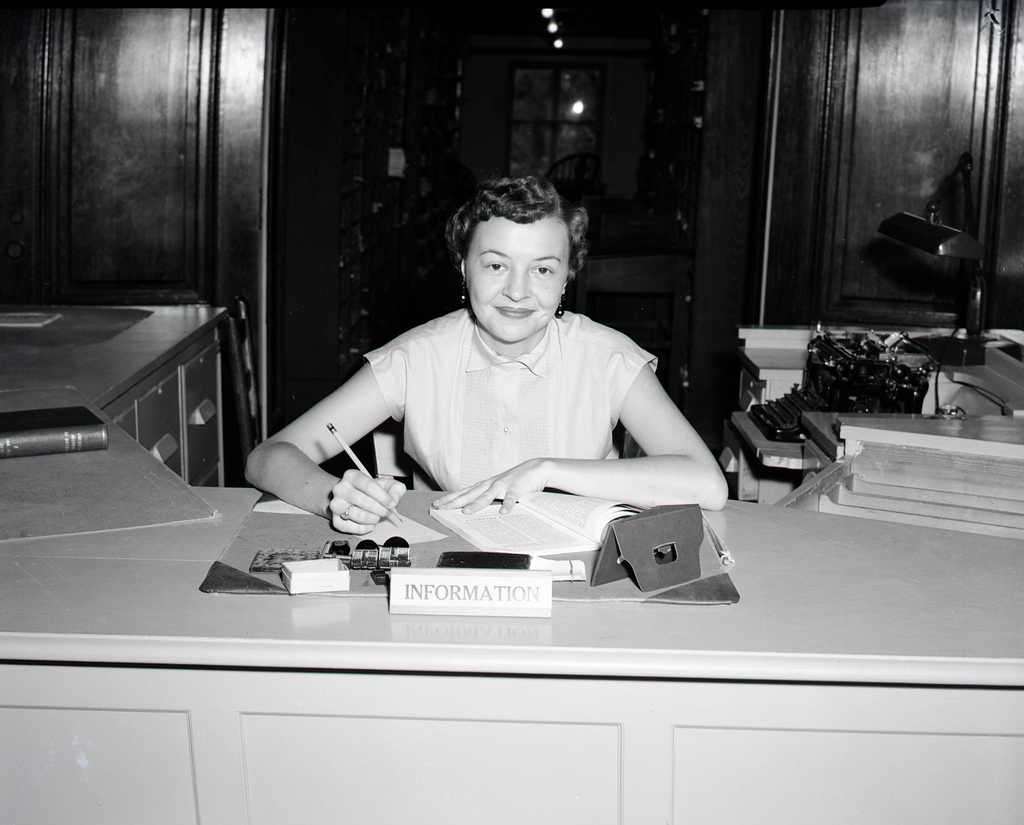
\includegraphics[height=7.5cm]{./pics/servicedesk2.jpg}
 \end{column}
 \begin{column}{0.45\textwidth}
     \begin{block}{Web interfaces}
        \begin{itemize}
            \item End user simplified interface
            \item Standard interface
            \item Smartphones interface
        \end{itemize}
    \end{block}

 \end{column}
\end{columns}






\end{frame}
\begin{frame}

    \frametitle{Service Desk: the interfaces 2/2}


 \begin{columns}
 \begin{column}{0.45\textwidth}
         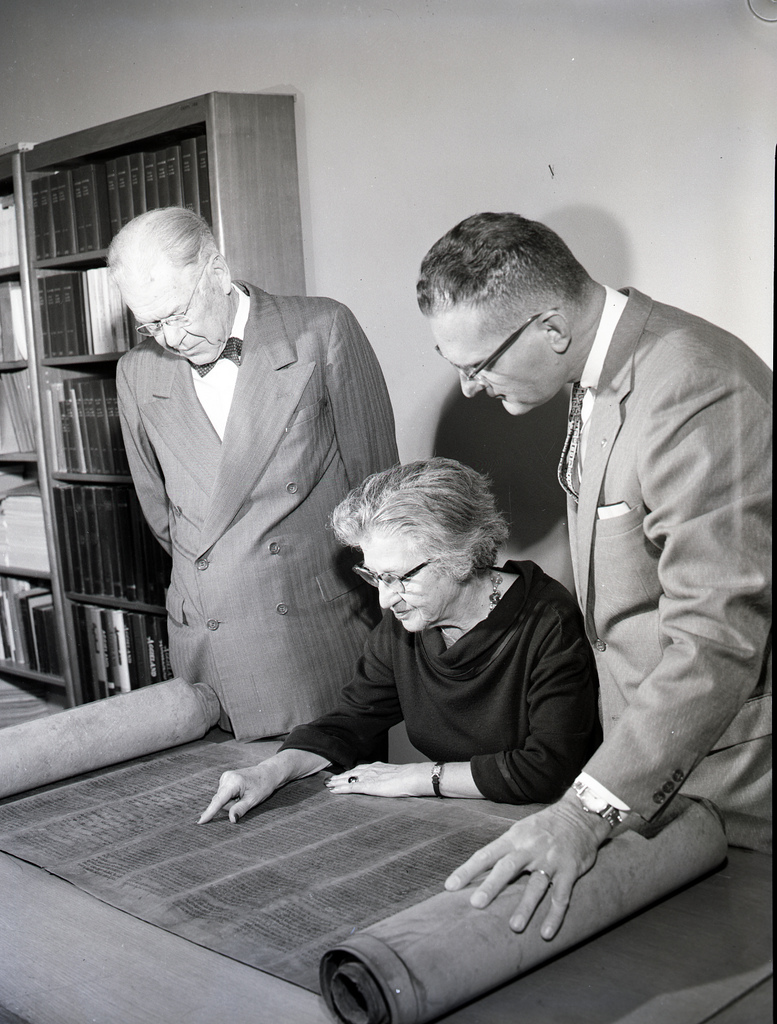
\includegraphics[height=7.5cm]{./pics/servicedesk3.jpg}
 \end{column}
 \begin{column}{0.45\textwidth}
     \begin{block}{Webservices}
        \begin{itemize}
            \item To integrate GLPI in another system
            \item To push tickets into another helpdesk software
            \item Or the opposite
        \end{itemize}
    \end{block}
\pause
    \begin{block}{Mail}
       \begin{itemize}
            \item Send notifications
            \item Add and update tickets
       \end{itemize}
    \end{block}


 \end{column}
\end{columns}

\end{frame}

\begin{frame}

\frametitle{Service Desk: reporting}
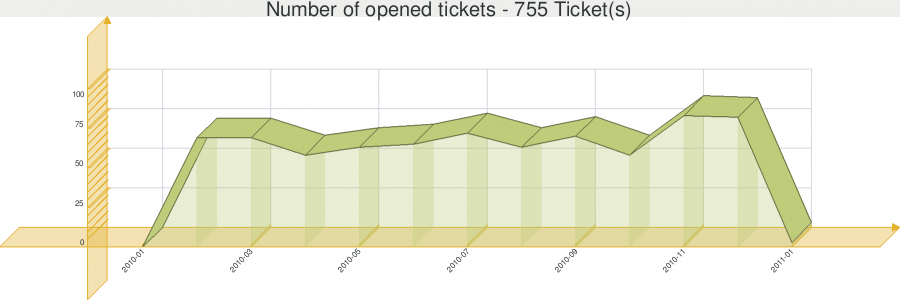
\includegraphics[height=3.5cm]{./pics/report1.png}
\end{frame}

\begin{frame}

    \frametitle{Application integration}
 \begin{columns}
 \begin{column}{0.45\textwidth}
         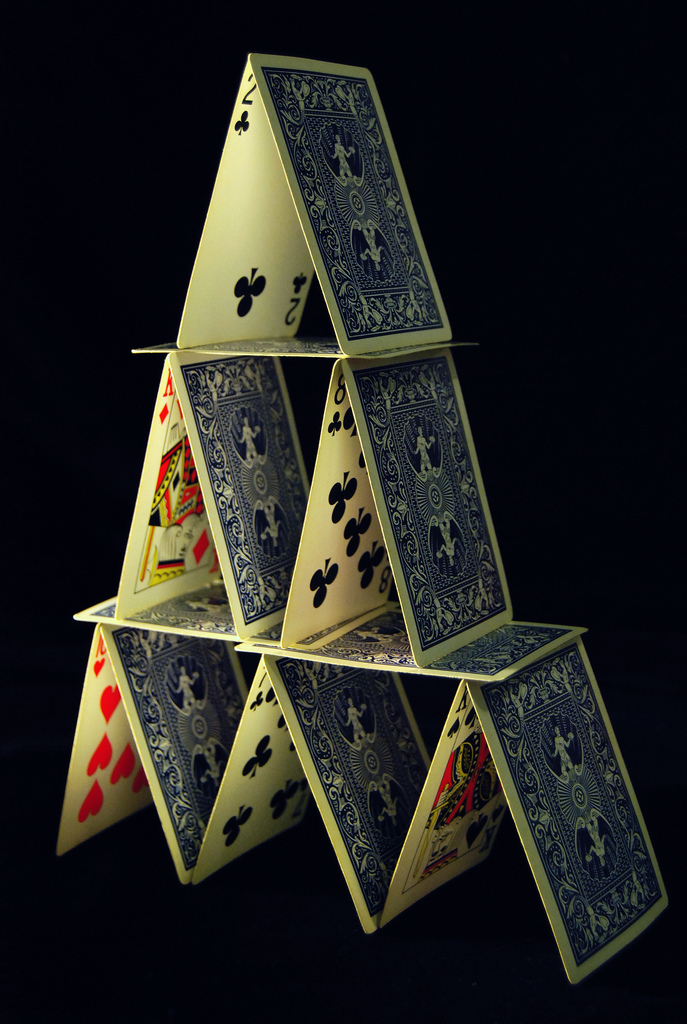
\includegraphics[height=7.5cm]{./pics/house_of_cards.jpg}
 \end{column}
 \begin{column}{0.45\textwidth}
     \begin{block}{Wait, some tools are already running here! \\
     How to interacte with them?}
        \begin{itemize}
            \item Webservice interface
            \item API for updates
            \item CSV import/export
        \end{itemize}
    \end{block}

 \end{column}
\end{columns}
\end{frame}



\section{GLPI plugins}

\begin{frame}

    \frametitle{The GLPI ecosystem}

 \begin{columns}
 \begin{column}{0.45\textwidth}
         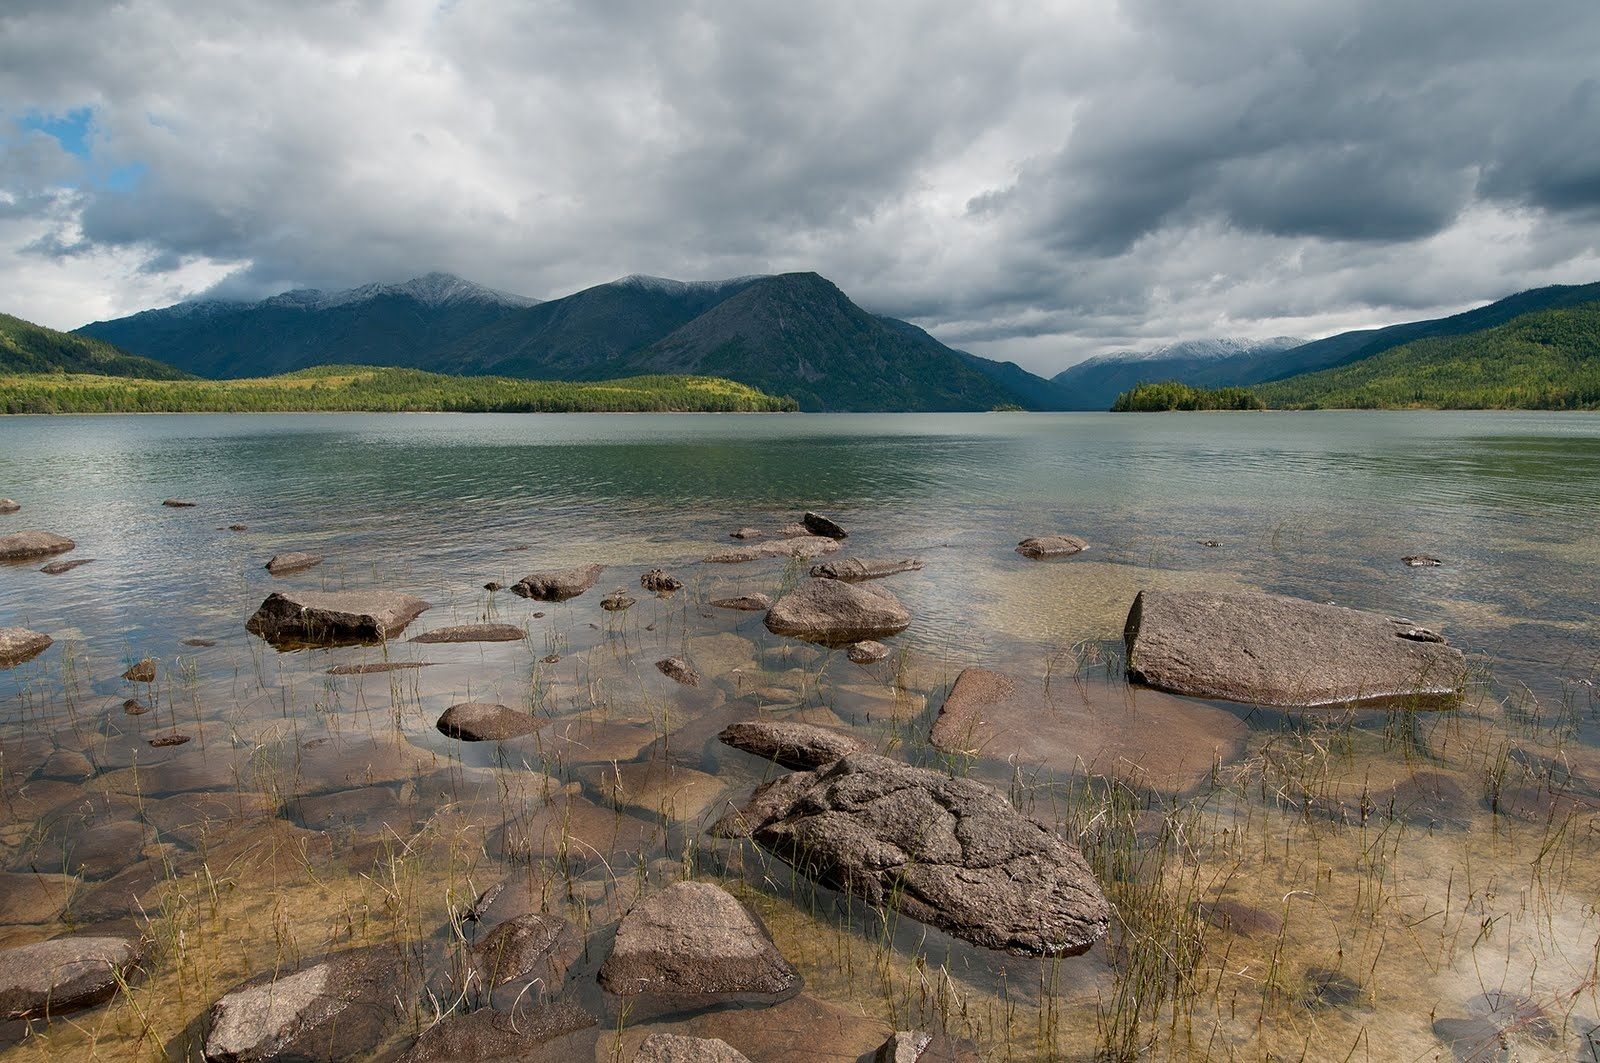
\includegraphics[height=7.5cm]{./pics/ecosystem.jpg}
 \end{column}
 \begin{column}{0.65\textwidth}
    \begin{block}{The ecosystem}
        \begin{itemize}
            \item A central interface
            \item A configuration database (CMDB)
            \item Various tools to collect information
            \item Additional features
        \end{itemize}
    \end{block}

 \end{column}
\end{columns}

\end{frame}




\begin{frame}

    \frametitle{\textbf{There is \sout{an app} a awesome plugin for that!}}

 \begin{columns}
 \begin{column}{0.45\textwidth}
         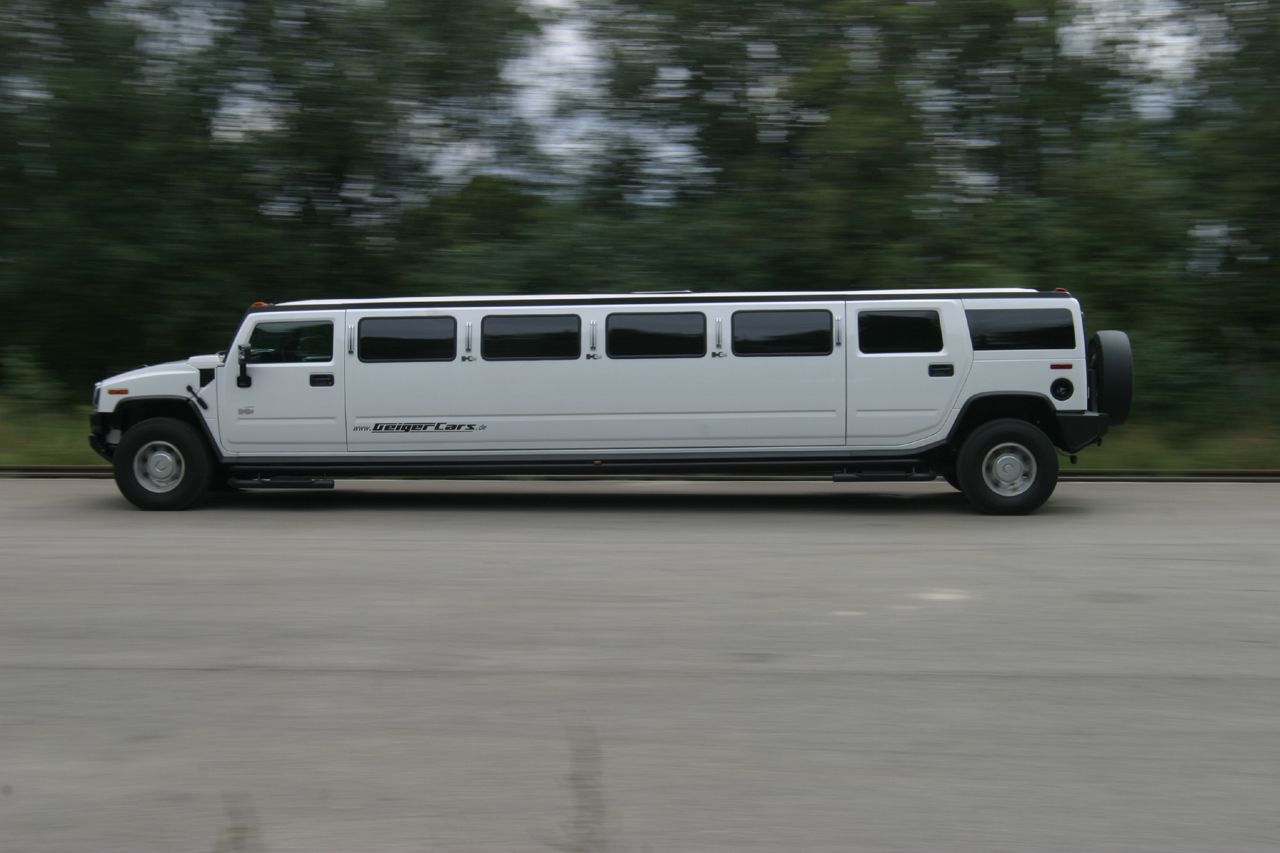
\includegraphics[height=7.5cm]{./pics/plugin.jpg}
 \end{column}
 \begin{column}{0.65\textwidth}
    \begin{block}{A large collection of \\
    extensions}
        \begin{itemize}
            \item Add load of new features
            \item Tight integration in GLPI
            \item Powerfull API
        \end{itemize}
    \end{block}

 \end{column}
\end{columns}

\end{frame}



\begin{frame}


    \frametitle{\textbf{There is \sout{an app} a plugin for that!}}

 \begin{columns}
 \begin{column}{0.45\textwidth}
         
\includegraphics[height=7.5cm]{./pics/nyancat.jpg}
         %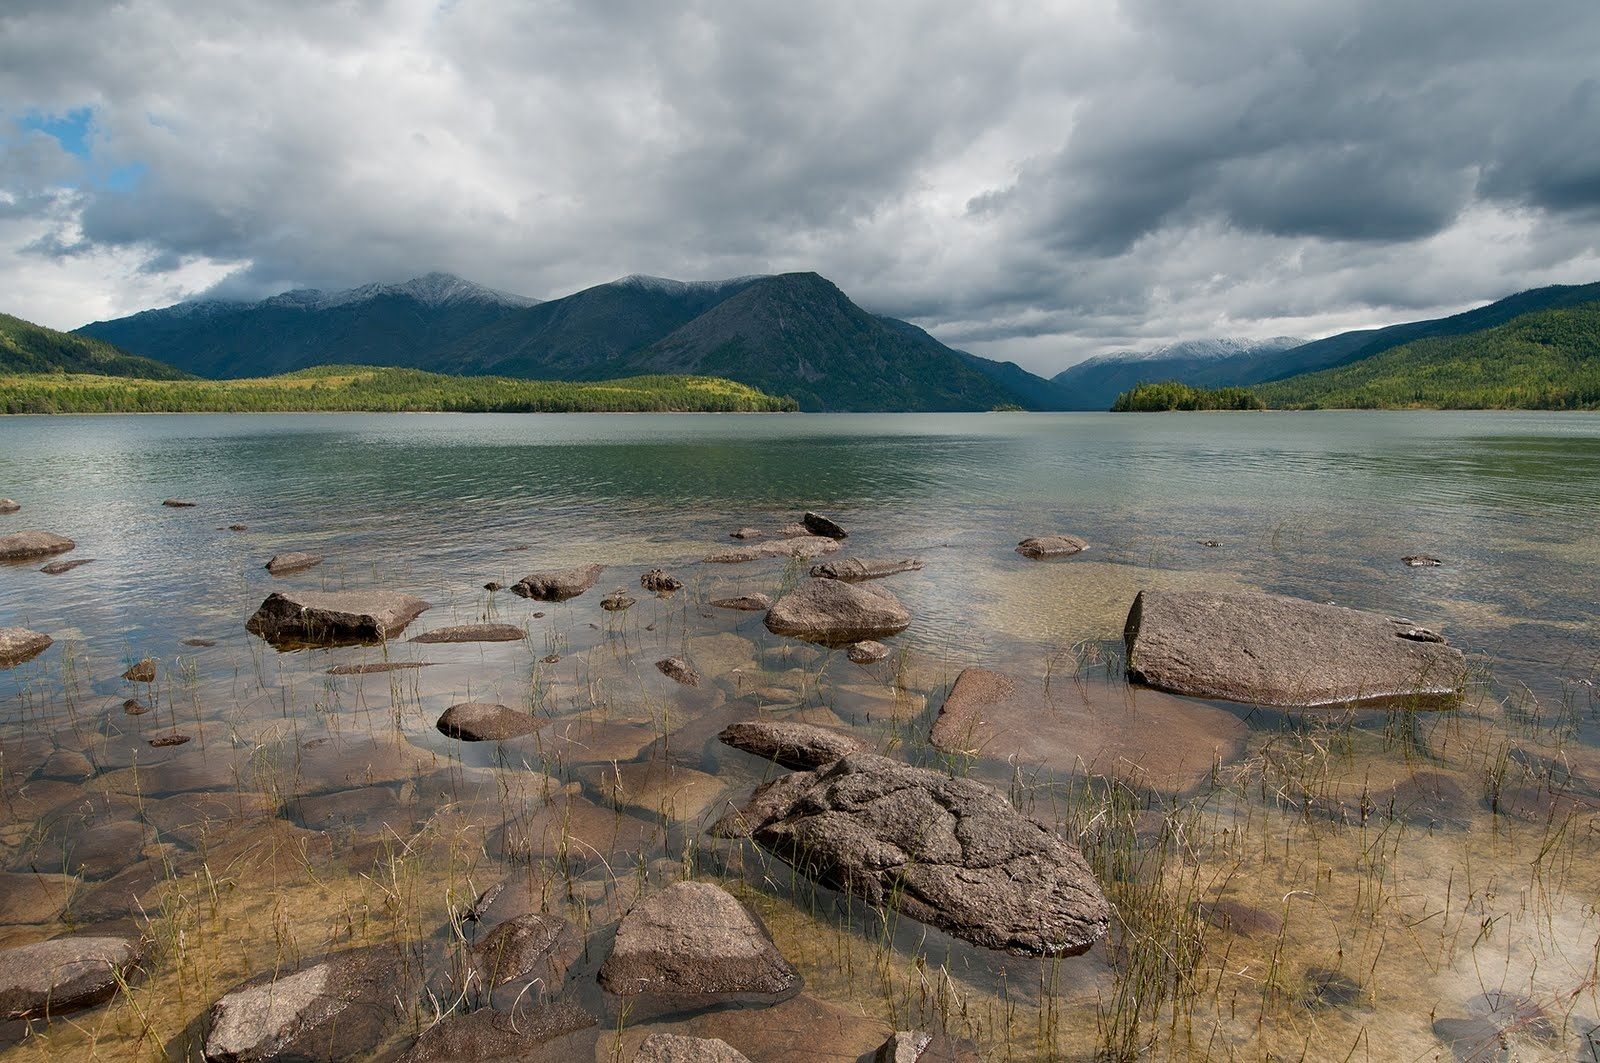
\includegraphics[height=7.5cm]{./pics/ecosystem.jpg}
 \end{column}
 \begin{column}{0.65\textwidth}
 \end{column}
\end{columns}

\end{frame}



\begin{frame}

    \frametitle{\textbf{There is \sout{an app} a plugin for that!}}

 \begin{columns}
 \begin{column}{0.45\textwidth}
         
\includegraphics[height=7.5cm]{./pics/nyancat.jpg}
         %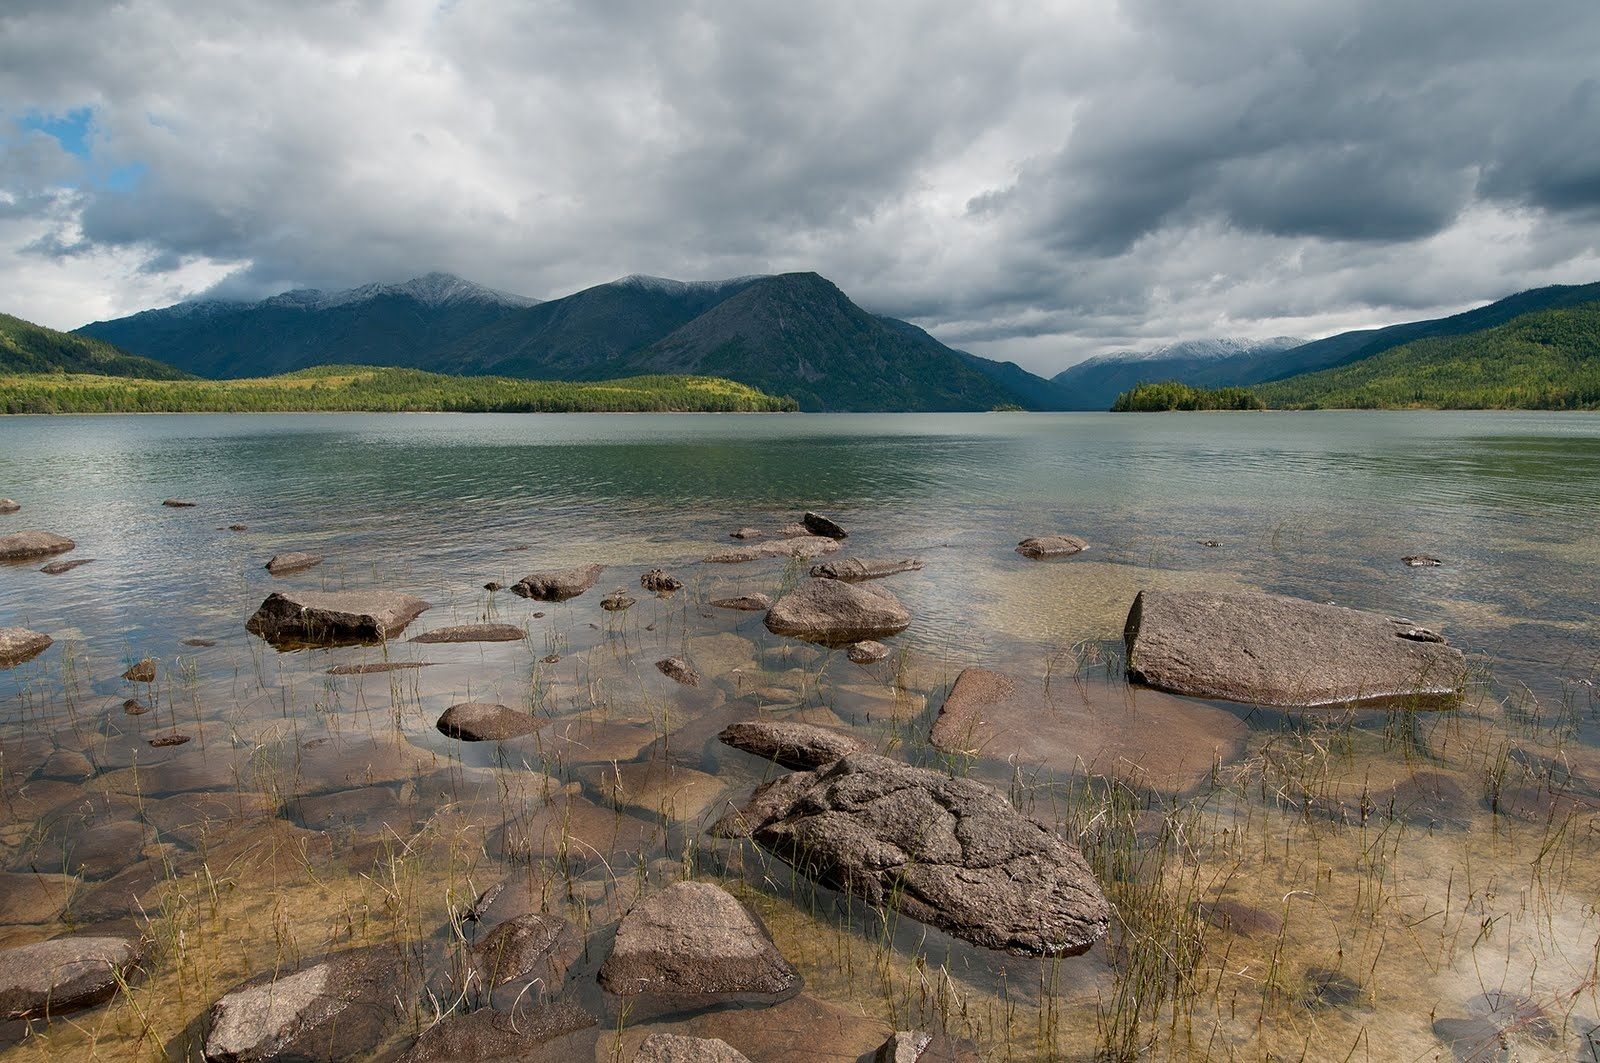
\includegraphics[height=7.5cm]{./pics/ecosystem.jpg}
 \end{column}
 \begin{column}{0.65\textwidth}
    \begin{block}{Plugins: Rules of Engagement}
        \begin{itemize}
            \item External contribution
            \item Not endorsed by the GLPI Project
            \item Depends on a given version of GLPI
            \pause
            \item \textbf{Take care on the plugin origin}
        \end{itemize}
    \end{block}

 \end{column}
\end{columns}

\end{frame}


\begin{frame}
    \frametitle{plugin: Mobile}

 \begin{columns}
\begin{column}{0.5\textwidth}
   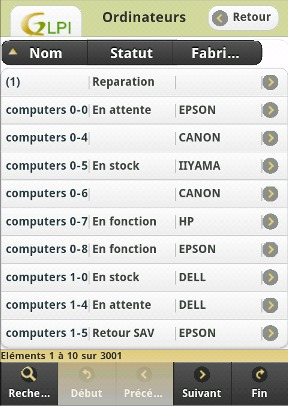
\includegraphics[height=3.5cm]{./pics/mobile/computers.jpg}
 \end{column}

 \begin{column}{0.5\textwidth}
   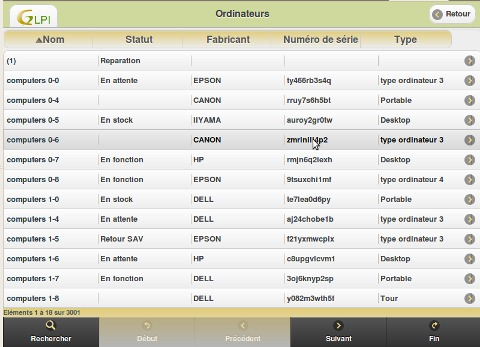
\includegraphics[height=3.5cm]{./pics/mobile/computers_tablet.jpg}
 \end{column}
\end{columns}

\end{frame}

\begin{frame}
    \frametitle{plugin: Mobile}

 \begin{columns}
 \begin{column}{0.5\textwidth}
 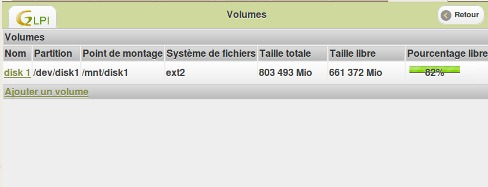
\includegraphics[height=3.5cm]{./pics/mobile/volumes_detail_tablet.jpg}
 \end{column}
 \begin{column}{0.5\textwidth}
   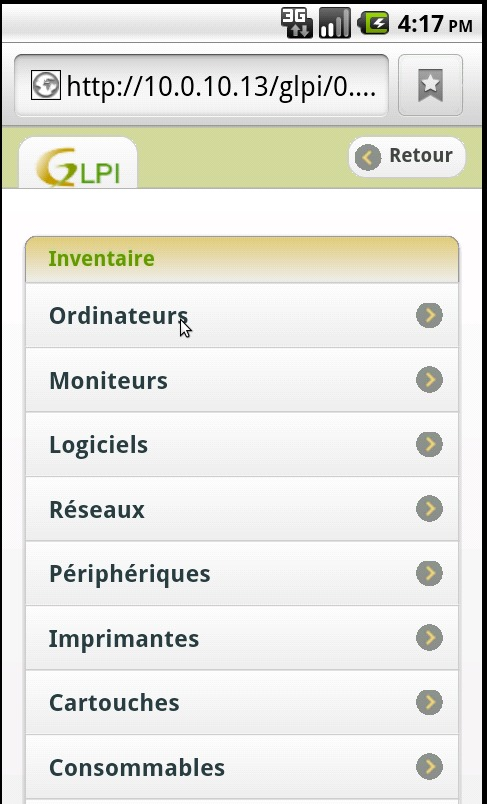
\includegraphics[height=3.5cm]{./pics/mobile/inventory.jpg}
 \end{column}
\end{columns}

\end{frame}

\begin{frame}
    \frametitle{plugin: Mobile}

 \begin{columns}
 \begin{column}{0.5\textwidth}
    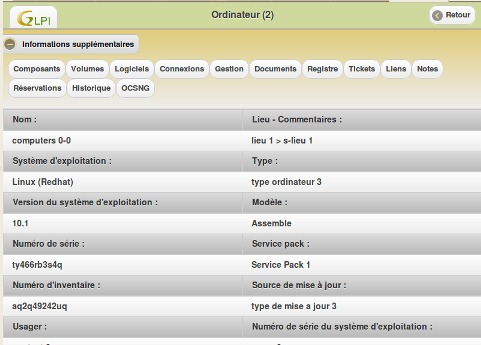
\includegraphics[height=3.5cm]{./pics/mobile/computer_detail_tablet.jpg}
 \end{column}
 \begin{column}{0.5\textwidth}
   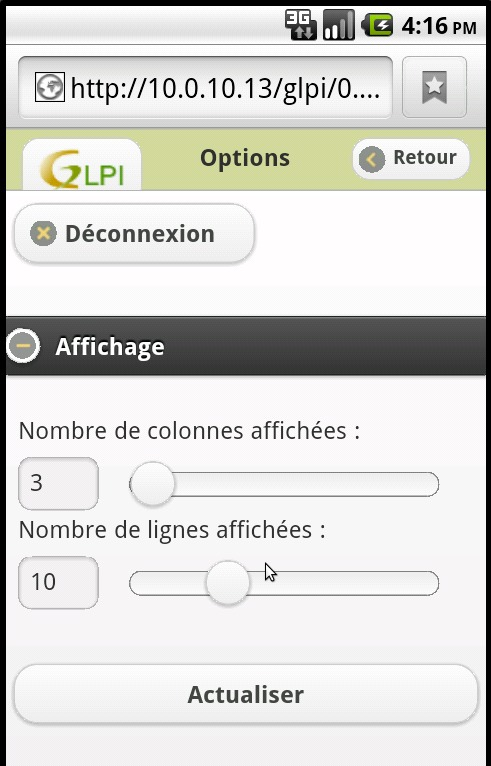
\includegraphics[height=3.5cm]{./pics/mobile/options.jpg}
 \end{column}
\end{columns}

\end{frame}



\begin{frame}
    \frametitle{plugin: FusionInventory}


    \begin{block}{
\includegraphics[height=0.5cm]{./pics/plugins/fusioninventory.jpg} FusionInventory}
        \begin{itemize}
            \item Import your computer
            \item Identify and import remote devices (switchs, printers, ..)
            \item VMware vCenter/ESX/ESXi remote inventory
            \item Wake on LAN
        \end{itemize}
    \end{block}

\end{frame}



\begin{frame}
    \frametitle{plugin: Multi-GLPI}

    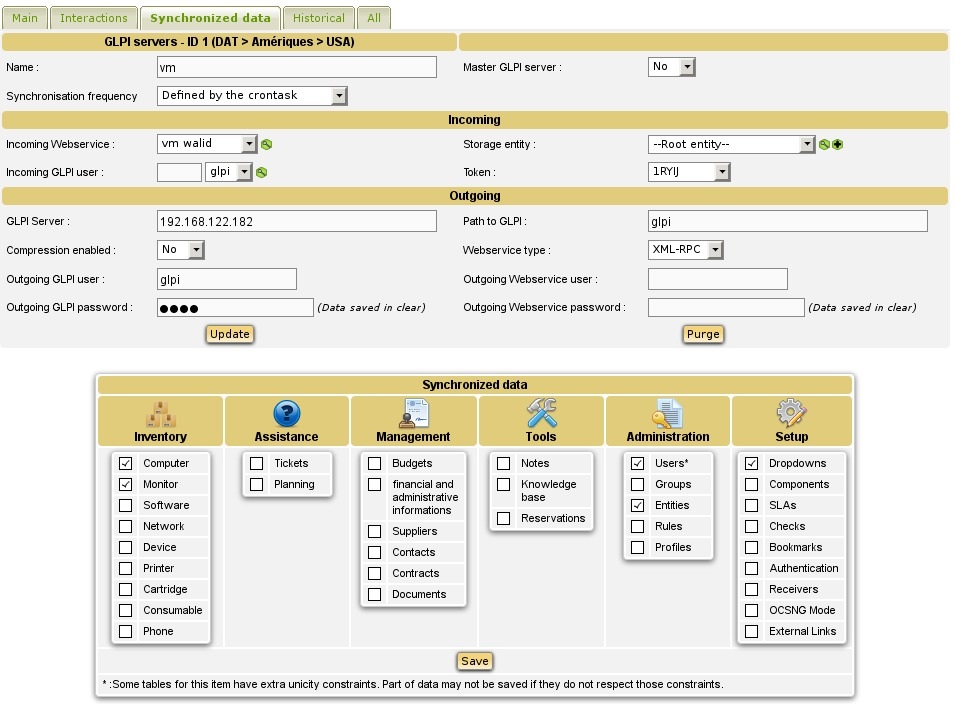
\includegraphics[height=7.5cm]{./pics/multiglpi/multiGLPi.jpg}




\end{frame}



\begin{frame}
    \frametitle{plugin: PDF}

    \begin{block}{
\includegraphics[height=0.5cm]{./pics/plugins/pdf.jpg} PDF}
        \begin{itemize}
            \item PDF export of a given inventory item
        \end{itemize}
    \end{block}

\end{frame}

\begin{frame}
    \frametitle{plugin: Behaviors}

    \begin{block}{
\includegraphics[height=0.5cm]{./pics/plugins/behaviors.jpg} Behaviors}
        Additional behaviors to GLPI.
        \begin{itemize}
            \item helpdesk (ticket own changes, ticket number format, etc)
            \item Inventory management
        \end{itemize}
    \end{block}

\end{frame}


\begin{frame}
    \frametitle{plugin: Order}

    \begin{block}{
\includegraphics[height=0.5cm]{./pics/plugins/order.jpg} Order}
        Order management
        \begin{itemize}
            \item Manage your order
            \item Products references management
            \item Validation workflow
        \end{itemize}
    \end{block}

\end{frame}


\begin{frame}
    \frametitle{plugin: Appliance}

    \begin{block}{
\includegraphics[height=0.5cm]{./pics/plugins/appliance.jpg} Appliance}
        Create element from a group of several item.
        \begin{itemize}
            \item Any kind of item
            \item Use them as any generic object
        \end{itemize}
    \end{block}

\end{frame}

\begin{frame}
    \frametitle{plugin: Account Inventory}

    \begin{block}{
\includegraphics[height=0.5cm]{./pics/plugins/account.jpg} Account Inventory}
        Manage and share the credentials between users.
        \begin{itemize}
            \item Attach a credential information to an item
            \item Credential expiration
            \item Mail system to check identity
        \end{itemize}
    \end{block}

\end{frame}

\begin{frame}
    \frametitle{plugin: Web Application}

    \begin{block}{
\includegraphics[height=0.5cm]{./pics/plugins/webapp.jpg} WebApplication}
        List web applications on your network and associate them with elements of the inventory.
    \end{block}

\end{frame}



\begin{frame}
    \frametitle{plugin: Human Resources Management}

    \begin{block}{
\includegraphics[height=0.5cm]{./pics/plugins/human.jpg} Human Resources Management}
        Trace user/assets affectation. eg: \\
        \small{This engineer is in the company for 3 months and we gave him 1 laptop and 1 screen. We need to remember to get them back.}
    \end{block}

\end{frame}


\begin{frame}
    \frametitle{plugin: Reports}

    \begin{block}{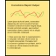
\includegraphics[height=0.5cm]{./pics/plugins/reports.jpg} Reports}
        Additional reports. It also allow you to add new reports in a simply way.
        \begin{itemize}
            \item Create your own reports
            \item A collection of ready to use reports
        \end{itemize}
    \end{block}

\end{frame}


\begin{frame}
    \frametitle{plugin: Mobile}
 \begin{columns}
 \begin{column}{0.55\textwidth}
    \begin{block}{
\includegraphics[height=0.5cm]{./pics/plugins/mobile.jpg}GLPI for mobile devices}
        \begin{itemize}
            \item iPhone/iPad
            \item Android
            \item Blackberry
            \item Windows Phone
        \end{itemize}
        GLPI 0.78 only for the moment.
    \end{block}

 \end{column}
 \begin{column}{0.1\textwidth}
 \end{column}
    \includegraphics[height=3.5cm]{./pics/mobile/central.jpg}

\end{columns}
\end{frame}

\begin{frame}
    \frametitle{plugin: Manufacturers Web Imports}

    \begin{block}{\includegraphics[height=0.5cm]{./pics/plugins/manufacturer.jpg} Manufacturers Web Imports}
        Imports financials and warranty informations directly from manufacturers web site.
        \begin{itemize}
            \item Dell
            \item HP
            \item Toshiba
            \item Fujitsu-Siemens
        \end{itemize}
    \end{block}

\end{frame}



\begin{frame}
    \frametitle{plugin: WebService}

    \begin{block}{\includegraphics[height=0.5cm]{./pics/plugins/webservice.jpg} WebService}
        Generic WebService interface for:
        \begin{itemize}
            \item SOAP
            \item XML/RPC
            \item REST
        \end{itemize}
        Can be used by other plugins to expose additional services.
    \end{block}

\end{frame}


\begin{frame}
    \frametitle{plugin: Monitoring}

    \begin{block}{Monitoring}
        Integration with Shinken monitoring solution.
        \begin{itemize}
            \item Define your services directly into GLPI.
            \item Device dependency.
            \item Display the alert.
            \item Create ticket on alert.
        \end{itemize}
    \end{block}
\WorkInProgress
\end{frame}


\begin{frame}
    \frametitle{plugin: Multi-GLPI}

    \begin{block}{\includegraphics[height=0.5cm]{./pics/plugins/multiglpi.jpg} Multi-GLPI}
        Synchronize serveral GLPI together.
        \begin{itemize}
            \item Master $\Longleftrightarrow$ Master GLPI
            \item Master $\Longleftrightarrow$ Master $\Longrightarrow$ Slaver $\Longrightarrow$ Slave
            \item ...
        \end{itemize}
    \end{block}


\WorkInProgress
\end{frame}


\begin{frame}
    \frametitle{plugin: OCSNG}


    \begin{block}{\includegraphics[height=0.5cm]{./pics/plugins/ocsinventory.jpg} OCS Inventory NG import}
        \begin{itemize}
            \item Import and synchronize computers from a OCS Inventory database
        \end{itemize}
    \end{block}

\end{frame}



\begin{frame}

    \frametitle{Newest features}

    \begin{block}{GLPI 0.80}
        \begin{itemize}
            \item SLA
            \item User satisfaction
            \item Link between ticket solution and knowledge base
            \item Multiple requesters, observers for a ticket
            \item Multiple technician, group and supplier assignement for a ticket
            \item Virtual machines management
        \end{itemize}
    \end{block}

\end{frame}

\begin{frame}

    \frametitle{Newest features}

    \begin{block}{GLPI 0.83}
        \begin{itemize}
            \item ITIL level 1 compliant until late 2011
            \item Problem management
            \item Change management
            \item Many more helpdesk improvements !
            \item OCSNG Mode available as a plugin
        \end{itemize}
    \end{block}

\end{frame}


\begin{frame}

    \frametitle{Computer}
 \begin{columns}
 \begin{column}{0.15\textwidth}
         \includegraphics[height=8.5cm]{./pics/os.pdf}
 \end{column}

 Use an system inventory solution.
 \begin{column}{1.25\textwidth}
    \begin{block}{Easy step}
        \begin{itemize}
            \item FusionInventory
            \item OCS Inventory
        \end{itemize}
    \end{block}


 \end{column}
\end{columns}
\end{frame}

\begin{frame}

    \frametitle{GLPI}

    \begin{block}{A nonprofit organisation}
        \begin{itemize}
            \item Indepnet, a french nonprofit association
            \item Since 2002
        \end{itemize}
    \end{block}

\end{frame}



\section{What else}

\begin{frame}

    \frametitle{What Else?}


\includegraphics[height=7.5cm]{./pics/whatelse.jpg}

\end{frame}



\begin{frame}

    \frametitle{GLPI}

    \begin{block}{A nonprofit organisation}
        \begin{itemize}
            \item Indepnet, a french nonprofit association
            \item Since 2002
        \end{itemize}
    \end{block}

\end{frame}





\begin{frame}

    \frametitle{GLPI}

    \begin{block}{Two independant projects leaders}
        \begin{itemize}
            \item Jean-Mathieu Doléans
            \item Julien Dombre
        \end{itemize}
    \end{block}
\pause
    \begin{block}{Contributors and developers}
        \begin{itemize}
            \item Developers and contributors
            \item Plugins developers
            \item Translators
        \end{itemize}
    \end{block}

\end{frame}

\begin{frame}

    \frametitle{GLPI}

 \begin{columns}
 \begin{column}{0.35\textwidth}
         \includegraphics[height=7.5cm]{./pics/agreement.jpg}
 \end{column}
 \begin{column}{0.65\textwidth}

    \begin{block}{GLPI Business partners}
        \begin{itemize}
            \item Agreement between the association and IT partners
            \item Partners bring money, support and code
        \end{itemize}
    \end{block}


 \end{column}
\end{columns}

\end{frame}

\section{Questions}

\begin{frame}
    \frametitle{Thanks}

        \begin{itemize}
                \item Purchasing: \url{http://www.flickr.com/photos/epsos/5394616925/}
                \item LDAP: \url{http://www.flickr.com/photos/heyrocker/2954514315/}
                \item SSO: \url{http://www.flickr.com/photos/13519089@N03/1380483002/}
                \item User picture: \url{http://www.flickr.com/photos/wonderlane/5043174502/}
                \item Manager: \url{http://www.flickr.com/photos/eastcapital/5228405457/}
                \item Server: \url{http://www.flickr.com/photos/sylvar/31436963/}
                \item Helpdesk: \url{http://www.flickr.com/photos/runlevel0/2196587153/}
                \item Database: \url{http://www.flickr.com/photos/garryknight/5476230085/}
                \item Information: \url{http://www.flickr.com/photos/garryknight/5476230085/}
                \item Networking: \url{http://www.flickr.com/photos/dbreg2007/4376127852/}
                \item Printer: \url{http://www.flickr.com/photos/photofarmer/467241015/}
                \item House of cards: \url{http://www.flickr.com/photos/gibbons/2294375187/in/photostream/}
                \item Sercice desk: \url{http://www.flickr.com/photos/cushinglibrary/4770917261/}
                \item Ecosystem: \url{http://www.fotopedia.com/items/picasaweb-5521382965365467090}
        \end{itemize}

\end{frame}


\end{document}
